% Options for packages loaded elsewhere
\PassOptionsToPackage{unicode}{hyperref}
\PassOptionsToPackage{hyphens}{url}
%
\documentclass[
  8pt,
  ignorenonframetext,
]{beamer}
\usepackage{pgfpages}
\setbeamertemplate{caption}[numbered]
\setbeamertemplate{caption label separator}{: }
\setbeamercolor{caption name}{fg=normal text.fg}
\beamertemplatenavigationsymbolsempty
% Prevent slide breaks in the middle of a paragraph
\widowpenalties 1 10000
\raggedbottom
\setbeamertemplate{part page}{
  \centering
  \begin{beamercolorbox}[sep=16pt,center]{part title}
    \usebeamerfont{part title}\insertpart\par
  \end{beamercolorbox}
}
\setbeamertemplate{section page}{
  \centering
  \begin{beamercolorbox}[sep=12pt,center]{part title}
    \usebeamerfont{section title}\insertsection\par
  \end{beamercolorbox}
}
\setbeamertemplate{subsection page}{
  \centering
  \begin{beamercolorbox}[sep=8pt,center]{part title}
    \usebeamerfont{subsection title}\insertsubsection\par
  \end{beamercolorbox}
}
\AtBeginPart{
  \frame{\partpage}
}
\AtBeginSection{
  \ifbibliography
  \else
    \frame{\sectionpage}
  \fi
}
\AtBeginSubsection{
  \frame{\subsectionpage}
}
\usepackage{amsmath,amssymb}
\usepackage{lmodern}
\usepackage{iftex}
\ifPDFTeX
  \usepackage[T1]{fontenc}
  \usepackage[utf8]{inputenc}
  \usepackage{textcomp} % provide euro and other symbols
\else % if luatex or xetex
  \usepackage{unicode-math}
  \defaultfontfeatures{Scale=MatchLowercase}
  \defaultfontfeatures[\rmfamily]{Ligatures=TeX,Scale=1}
\fi
% Use upquote if available, for straight quotes in verbatim environments
\IfFileExists{upquote.sty}{\usepackage{upquote}}{}
\IfFileExists{microtype.sty}{% use microtype if available
  \usepackage[]{microtype}
  \UseMicrotypeSet[protrusion]{basicmath} % disable protrusion for tt fonts
}{}
\makeatletter
\@ifundefined{KOMAClassName}{% if non-KOMA class
  \IfFileExists{parskip.sty}{%
    \usepackage{parskip}
  }{% else
    \setlength{\parindent}{0pt}
    \setlength{\parskip}{6pt plus 2pt minus 1pt}}
}{% if KOMA class
  \KOMAoptions{parskip=half}}
\makeatother
\usepackage{xcolor}
\newif\ifbibliography
\usepackage{color}
\usepackage{fancyvrb}
\newcommand{\VerbBar}{|}
\newcommand{\VERB}{\Verb[commandchars=\\\{\}]}
\DefineVerbatimEnvironment{Highlighting}{Verbatim}{commandchars=\\\{\}}
% Add ',fontsize=\small' for more characters per line
\usepackage{framed}
\definecolor{shadecolor}{RGB}{248,248,248}
\newenvironment{Shaded}{\begin{snugshade}}{\end{snugshade}}
\newcommand{\AlertTok}[1]{\textcolor[rgb]{0.94,0.16,0.16}{#1}}
\newcommand{\AnnotationTok}[1]{\textcolor[rgb]{0.56,0.35,0.01}{\textbf{\textit{#1}}}}
\newcommand{\AttributeTok}[1]{\textcolor[rgb]{0.77,0.63,0.00}{#1}}
\newcommand{\BaseNTok}[1]{\textcolor[rgb]{0.00,0.00,0.81}{#1}}
\newcommand{\BuiltInTok}[1]{#1}
\newcommand{\CharTok}[1]{\textcolor[rgb]{0.31,0.60,0.02}{#1}}
\newcommand{\CommentTok}[1]{\textcolor[rgb]{0.56,0.35,0.01}{\textit{#1}}}
\newcommand{\CommentVarTok}[1]{\textcolor[rgb]{0.56,0.35,0.01}{\textbf{\textit{#1}}}}
\newcommand{\ConstantTok}[1]{\textcolor[rgb]{0.00,0.00,0.00}{#1}}
\newcommand{\ControlFlowTok}[1]{\textcolor[rgb]{0.13,0.29,0.53}{\textbf{#1}}}
\newcommand{\DataTypeTok}[1]{\textcolor[rgb]{0.13,0.29,0.53}{#1}}
\newcommand{\DecValTok}[1]{\textcolor[rgb]{0.00,0.00,0.81}{#1}}
\newcommand{\DocumentationTok}[1]{\textcolor[rgb]{0.56,0.35,0.01}{\textbf{\textit{#1}}}}
\newcommand{\ErrorTok}[1]{\textcolor[rgb]{0.64,0.00,0.00}{\textbf{#1}}}
\newcommand{\ExtensionTok}[1]{#1}
\newcommand{\FloatTok}[1]{\textcolor[rgb]{0.00,0.00,0.81}{#1}}
\newcommand{\FunctionTok}[1]{\textcolor[rgb]{0.00,0.00,0.00}{#1}}
\newcommand{\ImportTok}[1]{#1}
\newcommand{\InformationTok}[1]{\textcolor[rgb]{0.56,0.35,0.01}{\textbf{\textit{#1}}}}
\newcommand{\KeywordTok}[1]{\textcolor[rgb]{0.13,0.29,0.53}{\textbf{#1}}}
\newcommand{\NormalTok}[1]{#1}
\newcommand{\OperatorTok}[1]{\textcolor[rgb]{0.81,0.36,0.00}{\textbf{#1}}}
\newcommand{\OtherTok}[1]{\textcolor[rgb]{0.56,0.35,0.01}{#1}}
\newcommand{\PreprocessorTok}[1]{\textcolor[rgb]{0.56,0.35,0.01}{\textit{#1}}}
\newcommand{\RegionMarkerTok}[1]{#1}
\newcommand{\SpecialCharTok}[1]{\textcolor[rgb]{0.00,0.00,0.00}{#1}}
\newcommand{\SpecialStringTok}[1]{\textcolor[rgb]{0.31,0.60,0.02}{#1}}
\newcommand{\StringTok}[1]{\textcolor[rgb]{0.31,0.60,0.02}{#1}}
\newcommand{\VariableTok}[1]{\textcolor[rgb]{0.00,0.00,0.00}{#1}}
\newcommand{\VerbatimStringTok}[1]{\textcolor[rgb]{0.31,0.60,0.02}{#1}}
\newcommand{\WarningTok}[1]{\textcolor[rgb]{0.56,0.35,0.01}{\textbf{\textit{#1}}}}
\setlength{\emergencystretch}{3em} % prevent overfull lines
\providecommand{\tightlist}{%
  \setlength{\itemsep}{0pt}\setlength{\parskip}{0pt}}
\setcounter{secnumdepth}{-\maxdimen} % remove section numbering
% type setting
% ------------------------------------------------------------------------------
\usepackage[german]{babel}     

% fonts
% ------------------------------------------------------------------------------
\usefonttheme{professionalfonts}

% slide title and horizontal line
% ------------------------------------------------------------------------------
\setbeamertemplate{frametitle}{%
    \vskip-30pt \color{black}\large%
    \begin{minipage}[b][23pt]{120mm}%
    \flushleft\insertframetitle%
    \end{minipage}%
}

\setbeamertemplate{headline}										
{
\vskip10pt\hfill\hspace{3.5mm} 										 
\vskip15pt\color{black}\rule{\textwidth}{0.4pt} 					 
}

% slide number
% ---------------------------------------------------------------
\setbeamertemplate{navigation symbols}{}
\setbeamertemplate{footline}
{
\vskip5pt
\vskip2pt
\makebox[123mm]{\hspace{7.5mm}
\hfill Allgemeines Lineares Modell $\vert$ 
\copyright $ $ 2023 Dirk Ostwald CC BY 4.0 $\vert$ 
Folie \insertframenumber}
\vskip4pt
}

% block color scheme
% ------------------------------------------------------------------------------
% colors
\definecolor{white}{RGB}{255,255,255}
\definecolor{grey}{RGB}{235,235,235}
\definecolor{lightgrey}{RGB}{245,245,245}
\definecolor{LightBlue}{RGB}{220,220,255}
\definecolor{darkblue}{RGB}{51, 51, 153}

% definitions and theorems
\setbeamercolor{block title}{fg = black, bg = grey}
\setbeamercolor{block body}{fg = black, bg = lightgrey}

% general line spacing 
% ------------------------------------------------------------------------------
\linespread{1.3}

% local line spacing
% ------------------------------------------------------------------------------
\usepackage{setspace}

% colors
% -----------------------------------------------------------------------------
\usepackage{color}

% justified text
% ------------------------------------------------------------------------------
\usepackage{ragged2e}
\usepackage{etoolbox}
\apptocmd{\frame}{}{\justifying}{}

% bullet point lists
% -----------------------------------------------------------------------------
\setbeamertemplate{itemize item}[circle]
\setbeamertemplate{itemize subitem}[circle]
\setbeamertemplate{itemize subsubitem}[circle]
\setbeamercolor{itemize item}{fg = black}
\setbeamercolor{itemize subitem}{fg = black}
\setbeamercolor{itemize subsubitem}{fg = black}
\setbeamercolor{enumerate item}{fg = black}
\setbeamercolor{enumerate subitem}{fg = black}
\setbeamercolor{enumerate subsubitem}{fg = black}
\setbeamerfont{itemize/enumerate body}{}
\setbeamerfont{itemize/enumerate subbody}{size = \normalsize}
\setbeamerfont{itemize/enumerate subsubbody}{size = \normalsize}

% color links
% ------------------------------------------------------------------------------
\usepackage{hyperref}
\definecolor{urls}{RGB}{204,0,0}
\hypersetup{colorlinks, citecolor = darkblue, urlcolor = urls}


% additional math commands
% ------------------------------------------------------------------------------
\usepackage{bm}                                         
\newcommand{\niton}{\not\owns}
\DeclareMathOperator*{\intinf}{\int_{-\infty}^{\infty}}


% text highlighting
% ------------------------------------------------------------------------------
\usepackage{soul}
\makeatletter
\let\HL\hl
\renewcommand\hl{%
  \let\set@color\beamerorig@set@color
  \let\reset@color\beamerorig@reset@color
  \HL}
\makeatother

% equation highlighting
% -----------------------------------------------------------------------------
\newcommand{\highlight}[2][yellow]{\mathchoice%
  {\colorbox{#1}{$\displaystyle#2$}}%
  {\colorbox{#1}{$\textstyle#2$}}%
  {\colorbox{#1}{$\scriptstyle#2$}}%
  {\colorbox{#1}{$\scriptscriptstyle#2$}}}%

% additional mathematical operators
% ------------------------------------------------------------------------------
\DeclareMathOperator*{\argmax}{arg\,max}
\DeclareMathOperator*{\argmin}{arg\,min}

\ifLuaTeX
  \usepackage{selnolig}  % disable illegal ligatures
\fi
\IfFileExists{bookmark.sty}{\usepackage{bookmark}}{\usepackage{hyperref}}
\IfFileExists{xurl.sty}{\usepackage{xurl}}{} % add URL line breaks if available
\urlstyle{same} % disable monospaced font for URLs
\hypersetup{
  hidelinks,
  pdfcreator={LaTeX via pandoc}}

\author{}
\date{\vspace{-2.5em}}

\begin{document}

\begin{frame}[plain]{}
\protect\hypertarget{section}{}
\center

\begin{center}
\includegraphics[width=0.2\linewidth]{5_Abbildungen/alm_5_otto} \end{center}

\vspace{2mm}

\huge

Allgemeines Lineares Modell \vspace{6mm}

\large

BSc Psychologie SoSe 2023

\vspace{6mm}
\normalsize

Prof.~Dr.~Dirk Ostwald
\end{frame}

\begin{frame}[plain]{}
\protect\hypertarget{section-1}{}
\center
\huge
\vfill

\noindent (5) Modellformulierung \vfill
\end{frame}

\begin{frame}{Überblick}
\protect\hypertarget{uxfcberblick}{}
\vspace{1mm}

\textcolor{darkblue}{Modul B2 Inferenzstatistik | Allgemeines Lineares Modell}
\small \center \footnotesize \renewcommand{\arraystretch}{1.1}

\begin{tabular}{lll}
Datum       & Einheit                       & Thema                                             \\\hline
13.04.2023  & Grundlagen                    & (1) Regression                                  \\
20.04.2023  & Grundlagen                    & (2) Korrelation                             \\
27.04.2023  & Grundlagen                    & (3) Matrizen                              \\
04.05.2023  & Grundlagen                    & (4) Normalverteilungen                    \\
11.05.2023  & Theorie                       & (5) Modellformulierung                    \\
\textcolor{gray}{18.05.2023}                &  \textcolor{gray}{Feiertag} &             \\  
25.05.2023  & Theorie                       & (6) Modellschätzung                       \\
01.06.2023  & Theorie                       & (7) T-Statistiken                         \\
08.06.2021  & Theorie                       & (8) F-Statistiken                         \\
15.06.2021  & Anwendung                     & (9) T-Tests                               \\
22.06.2021  & Anwendung                     & (10) Einfaktorielle Varianzanalyse        \\
29.06.2023  & Anwendung                     & (11) Zweifaktorielle Varianzanalyse       \\
06.07.2023  & Anwendung                     & (12) Multiple Regression                  \\
13.07.2023  & Anwendung                     & (13) Kovarianzanalyse                     \\\hline
20.07.2023  & Klausurtermin                 &                                           \\
März 2024   & Klausurwiederholungstermin    &
\end{tabular}
\end{frame}

\begin{frame}{}
\protect\hypertarget{section-2}{}
\large

Naturwissenschaft \vspace{7mm}

\begin{center}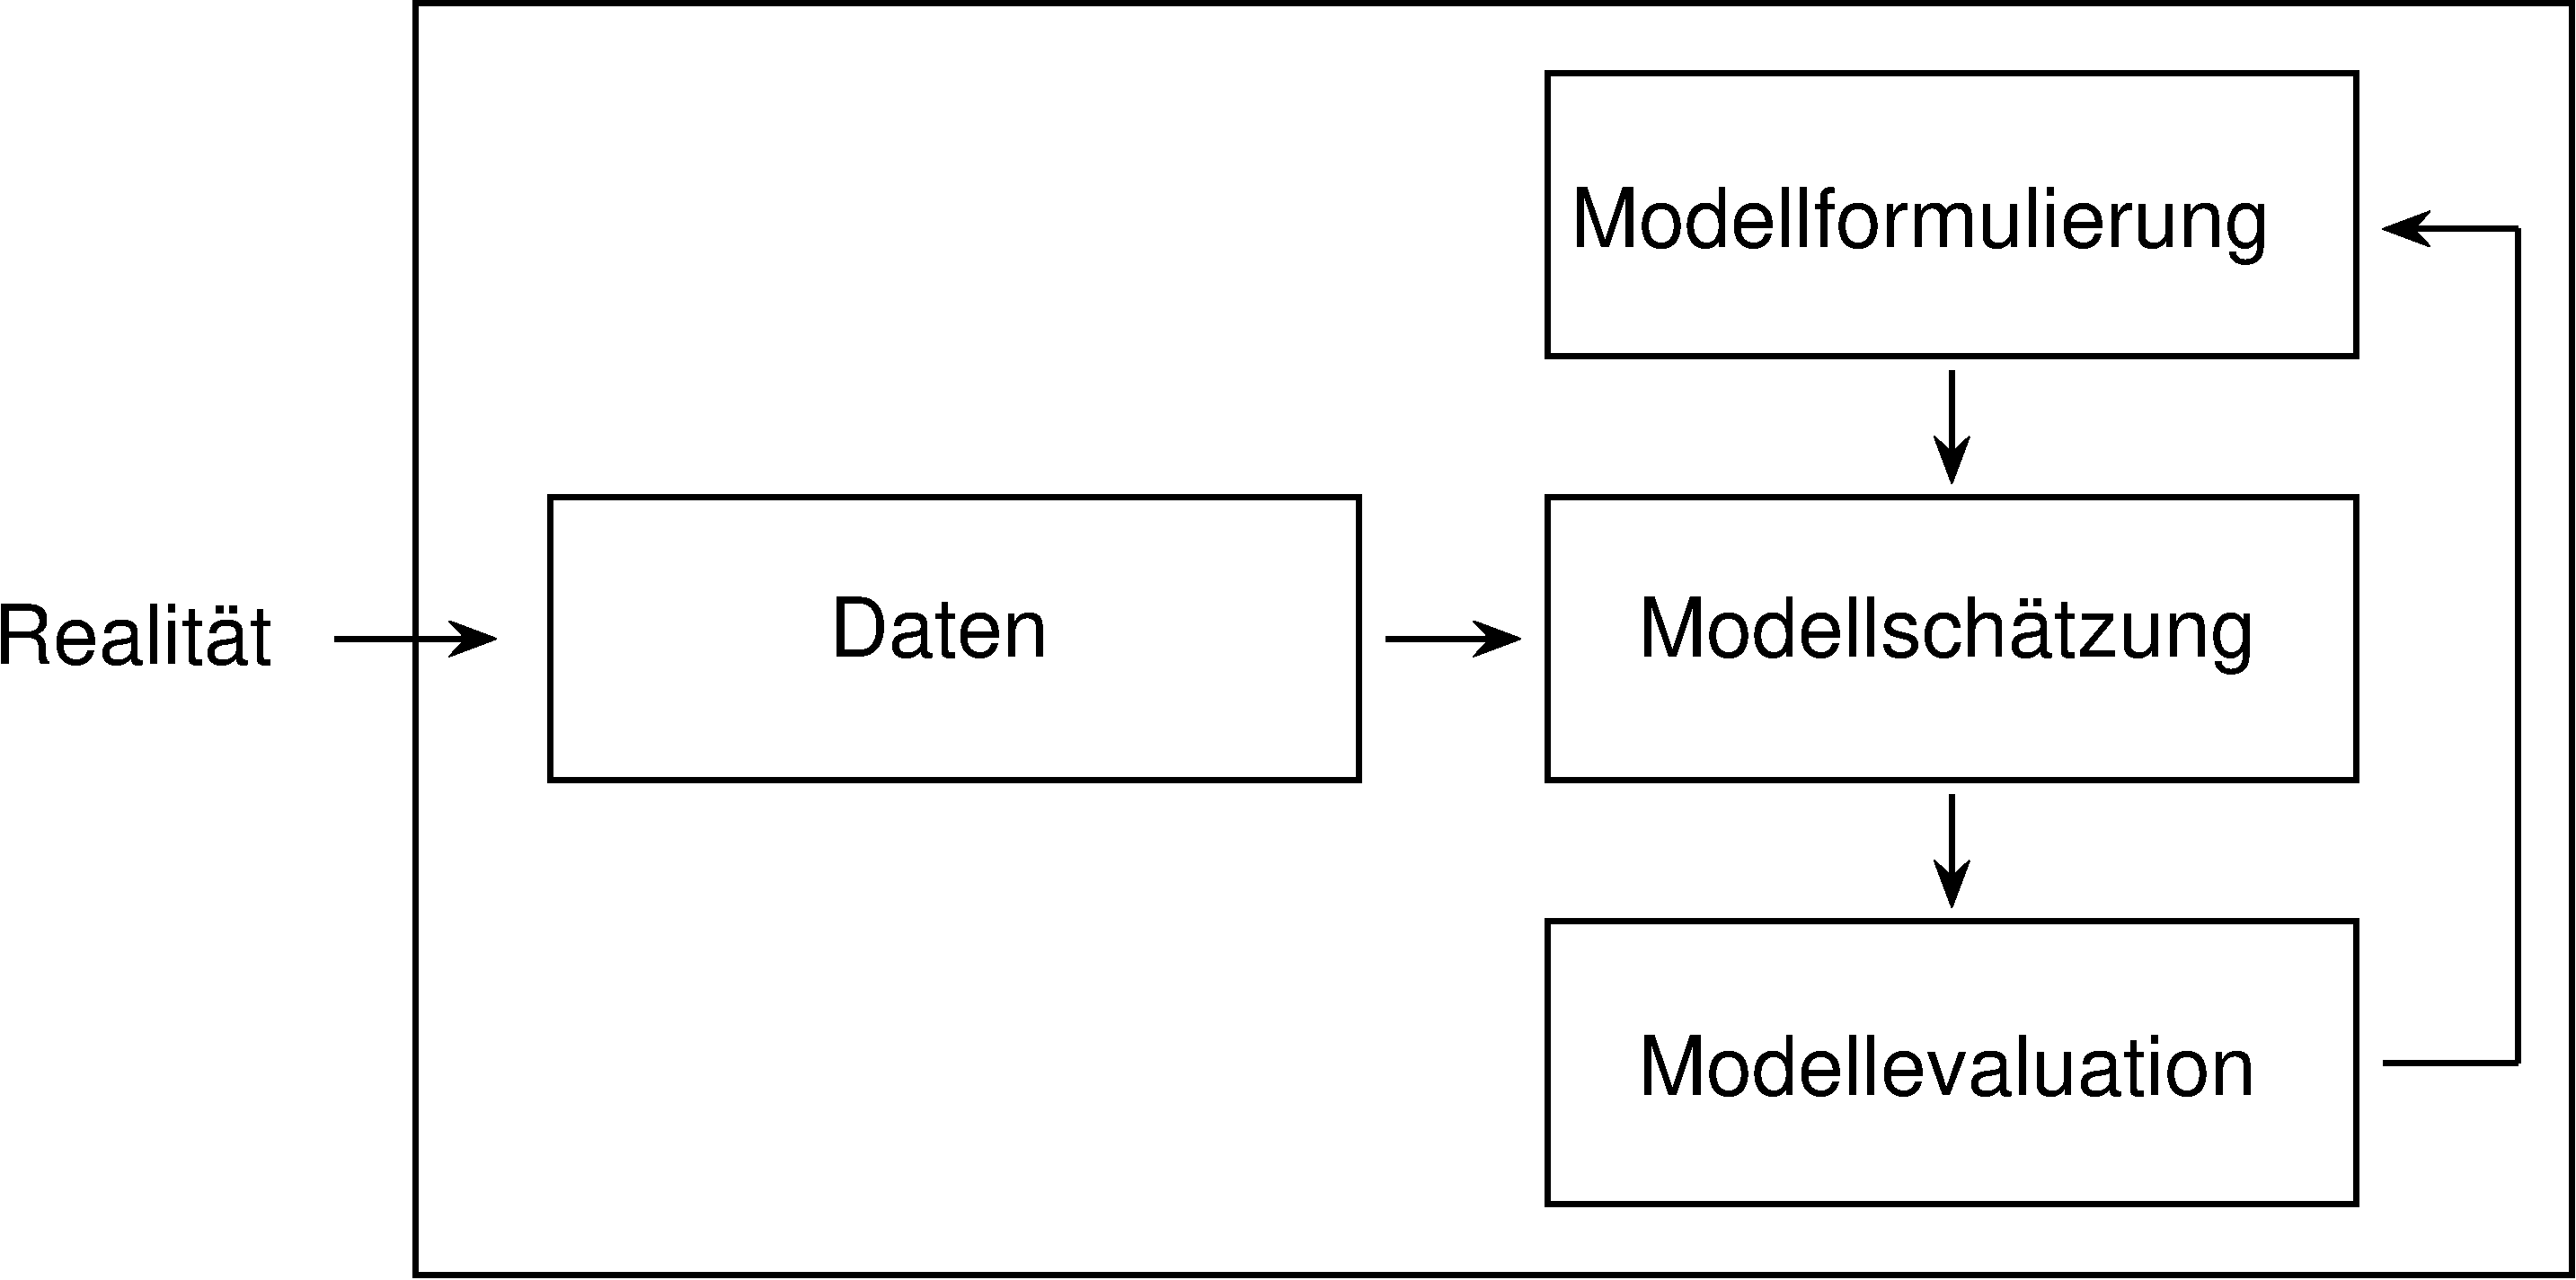
\includegraphics[width=0.9\linewidth]{5_Abbildungen/alm_5_wissenschaft} \end{center}
\end{frame}

\begin{frame}{}
\protect\hypertarget{section-3}{}
\vspace{1mm}
\normalsize

Modellformulierung \vspace{1mm} \small \begin{equation}
\upsilon = X\beta + \varepsilon, \varepsilon \sim N(0_n,\sigma^2I_n)
\end{equation} \vspace{5mm}

\normalsize

Modellschätzung \small \begin{equation}
\hat{\beta} = (X^TX)^{-1} X^T\upsilon,  \hat{\sigma}^2 = \frac{(\upsilon-X\hat{\beta})^T(\upsilon-X\hat{\beta})}{n-p}
\end{equation} \vspace{4mm}

\normalsize

Modellevaluation \small \begin{equation}
T = \frac{c^T\hat{\beta} - c^T\beta_0}{\sqrt{\hat{\sigma}^2c^T(X^TX)^{-1}c}},
F = \frac{(\hat{\varepsilon}_0^T\hat{\varepsilon}_0 - \hat{\varepsilon}^T\hat{\varepsilon})/p_1}{\hat{\varepsilon}^T\hat{\varepsilon}/(n-p)}
\end{equation}
\end{frame}

\begin{frame}{}
\protect\hypertarget{section-4}{}
Standardprobleme Frequentistischer Inferenz

\small
\vspace{2mm}

\noindent (1) Parameterschätzung

Ziel der Parameterschätzung ist es, einen möglichst guten Tipp für
wahre, aber unbekannte, Parameterwerte oder Funktionen dieser abzugeben,
typischerweise mithilfe von Daten.

\vspace{2mm}

\noindent (2) Konfidenzintervalle

Ziel der Bestimmung von Konfidenzintervallen ist es, basierend auf der
angenommenen Verteilung der Daten eine quantitative Aussage über die mit
Schätzwerten assoziierte Unsicherheit zu treffen.

\vspace{2mm}

\noindent (3) Hypothesentests

Ziel des Hypothesentestens ist es, basierend auf der angenommenen
Verteilung der Daten in einer möglichst zuverlässigen Form zu
entscheiden, ob ein wahrer, aber unbekannter Parameterwert in einer von
zwei sich gegenseitig ausschließenden Untermengen des Parameterraumes
liegt.
\end{frame}

\begin{frame}{}
\protect\hypertarget{section-5}{}
\center

\begin{center}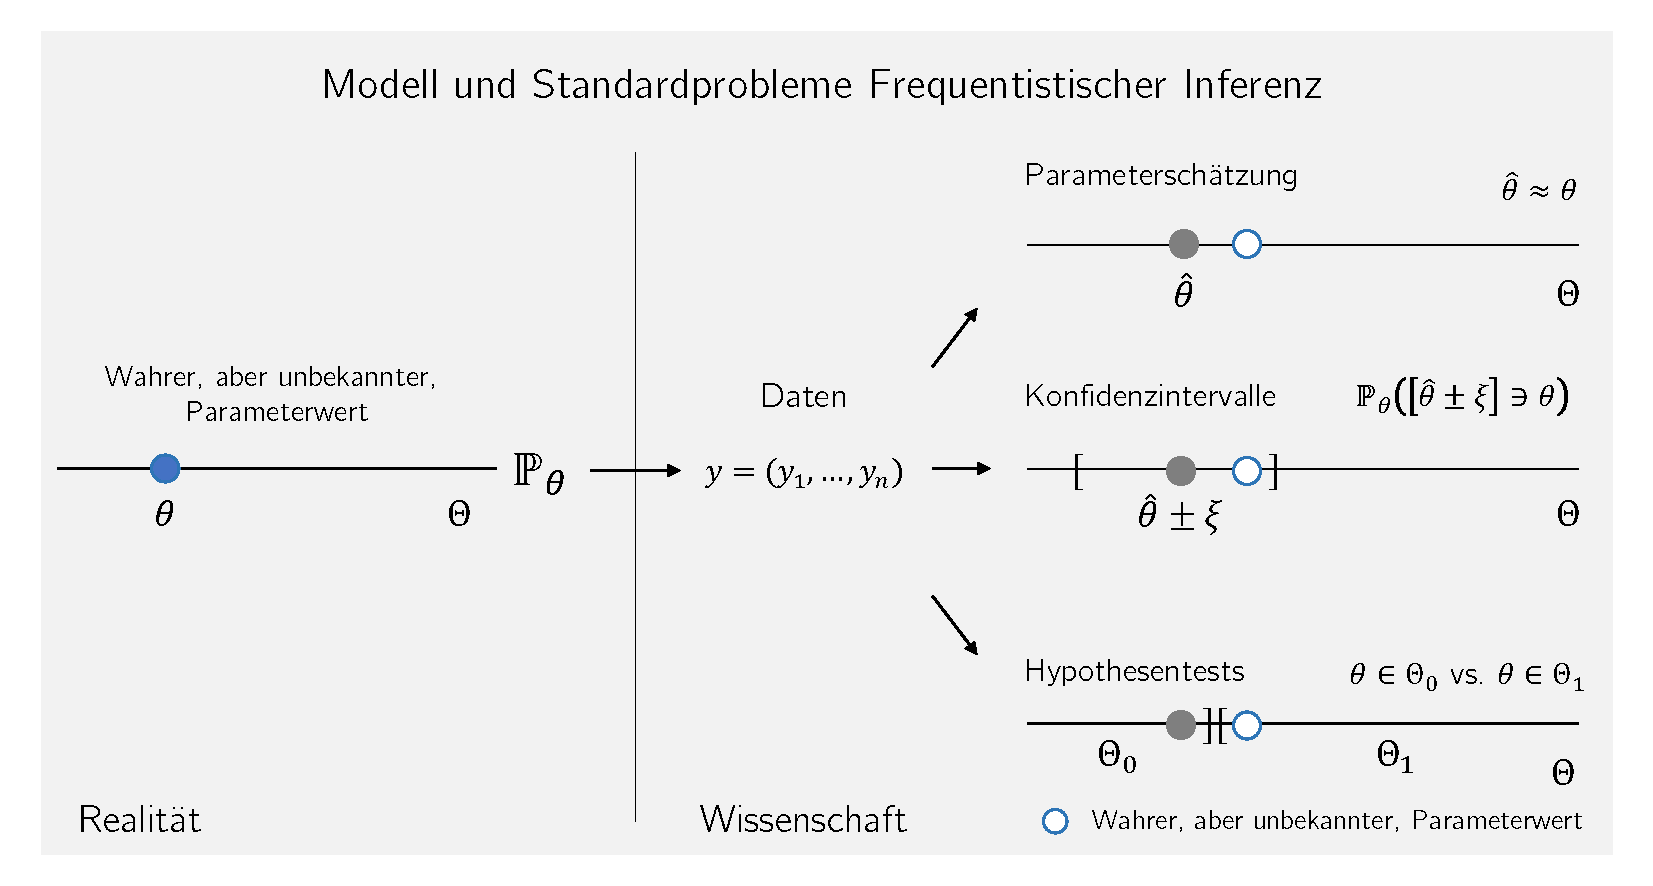
\includegraphics[width=1\linewidth]{5_Abbildungen/alm_5_frequentistische_inferenz} \end{center}
\center
\footnotesize

\(\theta := (\beta,\sigma^2)\),
\(\Theta := \mathbb{R}^p \times \mathbb{R}_{>0}\)
\(\mathbb{P}_\theta(\upsilon) := \mathbb{P}_{\beta,\sigma^2}(\upsilon)\)
mit WDF \(p_{\beta,\sigma^2}(y) := N(y;X\beta,\sigma^2I_n)\)
\end{frame}

\begin{frame}{}
\protect\hypertarget{section-6}{}
\small

Standardannahmen Frequentistischer Inferenz

\footnotesize
\setstretch{1.2}

Gegeben sei das Allgemeine Lineare Modell. Es wird angenommen, dass ein
vorliegender Datensatz eine der möglichen Realisierungen der Daten des
Modells ist. Aus Frequentistischer Sicht kann man unendlich oft
Datensätze basierend auf einem Modell generieren und zu jedem Datensatz
Schätzer oder Statistiken auswerten, z.B. den Betaparameterschätzer
\vspace{1mm}

\begin{itemize}
\item[] Datensatz (1) : $y^{(1)} = \left(y_1^{(1)}, y_2^{(1)}, ...,y_n^{(1)}\right)^T$  mit $\hat{\beta}^{(1)} = (X^TX)^{-1}X^Ty^{(1)}$
\item[] Datensatz (2) : $y^{(2)} = \left(y_1^{(2)}, y_2^{(2)}, ...,y_n^{(2)}\right)^T$  mit $\hat{\beta}^{(2)} = (X^TX)^{-1}X^Ty^{(2)}$
\item[] Datensatz (3) : $y^{(3)} = \left(y_1^{(3)}, y_2^{(3)}, ...,y_n^{(3)}\right)^T$  mit $\hat{\beta}^{(3)} = (X^TX)^{-1}X^Ty^{(3)}$
\item[] Datensatz (4) : $y^{(4)} = \left(y_1^{(4)}, y_2^{(4)}, ...,y_n^{(4)}\right)^T$  mit $\hat{\beta}^{(4)} = (X^TX)^{-1}X^Ty^{(4)}$
\item[] Datensatz (5) : $y^{(5)} = ...$
\end{itemize}

\vspace{1mm}

Um die Qualität statistischer Methoden zu beurteilen betrachtet die
Frequentistische Statistik die Wahrscheinlichkeitsverteilungen von
Schätzern und Statistiken unter Annahme der Datenverteilung. Was zum
Beispiel ist die Verteilung von \(\hat{\beta}^{(1)}\),
\(\hat{\beta}^{(2)}\), \(\hat{\beta}^{(3)}\), \(\hat{\beta}^{(4)}\),
\ldots{} also die Verteilung der Zufallsvariable
\(\hat{\beta} := (X^TX)^{-1}X^T\upsilon\)? Wenn eine statistische
Methode im Sinne der Frequentistischen Standardannahmen ``gut'' ist,
dann heißt das also, dass sie bei häufiger Anwendung ``im Mittel gut''
ist. Im Einzelfall, also im Normalfall nur eines vorliegenden
Datensatzes, kann sie auch ``schlecht'' sein.
\end{frame}

\begin{frame}{Überblick}
\protect\hypertarget{uxfcberblick-1}{}
\setstretch{2}

Anwendungsbeispiele Einheiten (5) - (8)

\begin{itemize}
\tightlist
\item
  Unabhängig und identisch normalverteilte Zufallsvariablen \textbar{}
  Einstichproben-T-Test
\item
  Einfache lineare Regression
\end{itemize}

Anwendungsbeispiele Einheiten (9) - (13)

\begin{itemize}
\tightlist
\item
  Zweistichproben-T-Tests
\item
  Einfaktorielle Varianzanalyse
\item
  Zweifaktorielle Varianzanalyse
\item
  Multiple Regression
\item
  Kovarianzanalyse
\end{itemize}
\end{frame}

\begin{frame}{}
\protect\hypertarget{section-7}{}
\large
\setstretch{3}
\vfill

Allgemeine Theorie

Unabhängige und identisch normalverteilte Zufallsvariablen

Einfache lineare Regression

Selbstkontrollfragen \vfill
\end{frame}

\begin{frame}{}
\protect\hypertarget{section-8}{}
\large
\setstretch{3}
\vfill

\textbf{Allgemeine Theorie}

Unabhängige und identisch normalverteilte Zufallsvariablen

Einfache lineare Regression

Selbstkontrollfragen \vfill
\end{frame}

\begin{frame}{Allgemeine Theorie}
\protect\hypertarget{allgemeine-theorie}{}
\small
\begin{definition}[Allgemeines Lineares Modell]
Es sei
\begin{equation}\label{eq:alm}
\upsilon = X\beta + \varepsilon, 
\end{equation}
wobei
\begin{itemize}
\item $\upsilon$ ein $n$-dimensionaler beobachtbarer Zufallsvektor ist, der \textit{Daten} genannt wird,
\item $X \in \mathbb{R}^{n \times p}$ mit $n>p$ eine vorgegebene Matrix ist, die \textit{Designmatrix} genannt wird,
\item $\beta \in \mathbb{R}^p$ ein unbekannter Parametervektor ist, der \textit{Betaparametervektor} genannt wird, 
\item $\varepsilon$ ein $n$-dimensionaler nicht-beobachtbarer Zufallsvektor ist, der \textit{Zufallsfehler} genannt wird und für den angenommen wird, dass
mit einem unbekannten Varianzparameter $\sigma^2>0$ gilt, dass
\begin{equation}
\varepsilon \sim N\left(0_n, \sigma^2I_n\right).
\end{equation}
\end{itemize}
Dann heißt \eqref{eq:alm} \textit{Allgemeines Lineares Modell (ALM)}.
\end{definition}
\end{frame}

\begin{frame}{Allgemeine Theorie}
\protect\hypertarget{allgemeine-theorie-1}{}
\footnotesize

Bemerkungen \setstretch{1.8}

\begin{itemize}
\tightlist
\item
  \justifying Wir nehmen durchgängig an, dass
  \(X \in \mathbb{R}^{n \times p}\) vollen Spaltenrang hat, also dass
  \(\mbox{rg}(X)=p\).
\item
  \(\upsilon\) ist ein Zufallsvektor, weil er aus der Addition des
  Zufallsvektors \(\varepsilon\) zu dem Vektor
  \(X\beta \in \mathbb{R}^n\) resultiert.
\item
  Wir nennen \(X\beta \in \mathbb{R}^n\) den
  \textit{deterministischen Modellaspekt} und \(\varepsilon\) den
  \textit{probabilistischen Modellaspekt}.
\item
  \(n \in \mathbb{N}\) bezeichnet durchgängig die Anzahl an
  Datenpunkten.
\item
  \(p \in \mathbb{N}\) bezeichnet durchgängig die Anzahl an
  Betaparametern.
\item
  Die Gesamtzahl an Parametern des ALMs ist \(p + 1\) (\(p\)
  Betaparameterkomponenten und \(1\) Varianzparameter).
\item
  Der Betaparametervektor wird auch \textit{Gewichtsvektor} oder
  \textit{Effektvektor} genannt.
\item
  Weil der Kovarianzmatrixparameter von \(\varepsilon\) als sphärisch
  angenommen wird, sind die \(\varepsilon_1,...,\varepsilon_n\)
  unabhängige normalverteilte Zufallsvariablen mit identischem
  Varianzparameter; weil zusätzlich der Erwartungswertparameter von
  \(\varepsilon\) als \(0_n\) angenommen wird, sind die
  \(\varepsilon_1,...,\varepsilon_n\) auch identisch normalverteilte
  Zufallsvariablen.
\item
  Für jede Komponente \(\upsilon_i, i = 1,...,n\) von \(\upsilon\)
  impliziert \eqref{eq:alm} nach Definition des Matrixprodukts, dass
  \begin{equation}
  \upsilon_i = x_{i1}\beta_1 + x_{i2}\beta_2 + \cdots +  x_{ip}\beta_p + \varepsilon_i \mbox{ mit } \varepsilon_i \sim N\left(0,\sigma^2\right),
  \end{equation} wobei \(x_{ij} \in \mathbb{R}\) das \(ij\)te Element
  der Designmatrix \(X\) bezeichnet.
\end{itemize}
\end{frame}

\begin{frame}{Allgemeine Theorie}
\protect\hypertarget{allgemeine-theorie-2}{}
\footnotesize
\begin{theorem}[Datenverteilung des Allgemeinen Linearen Modells]
\justifying
\normalfont
Es sei
\begin{equation}
\upsilon = X\beta + \varepsilon \mbox{ mit } \varepsilon \sim N(0_n,\sigma^2I_n)
\end{equation}
das ALM. Dann gilt
\begin{equation}
\upsilon \sim N(\mu,\sigma^2I_n) \mbox{ mit } \mu := X\beta \in \mathbb{R}^n.
\end{equation}
\end{theorem}

\underline{Beweis}

Mit dem Theorem zur linear-affinen Transformation multivariater
Normalverteilungen gilt für \(\varepsilon \sim N(0_n,\sigma^2I_n)\) und
\(\upsilon := I_n\varepsilon + X\beta\), dass \begin{equation}
\upsilon \sim N\left(I_n0_n + X\beta, I_n (\sigma^2 I_n) I_n^T\right) = N(X\beta, \sigma^2 I_n) = N(\mu,\sigma^2I_n) \mbox{ mit } \mu := X\beta \in \mathbb{R}^n.
\end{equation} Bemerkungen

\begin{itemize}
\tightlist
\item
  \justifying Im ALM sind die Daten \(\upsilon\) also ein
  \(n\)-dimensionaler normalverteilter Zufallsvektor mit
  Erwartungswertparameter \(\mu = X\beta \in \mathbb{R}^n\) und
  Kovarianzmatrixparameter \(\sigma^2I_n \in \mathbb{R}^{n \times n}\).
\item
  Die Komponenten \(\upsilon_1,...,\upsilon_n\) von \(\upsilon\), also
  die Datenpunkte, sind damit unabhängige, aber im Allgemeinen nicht
  identisch verteilte, normalverteilte Zufallsvariablen der Form
  \(\upsilon_i \sim N\left(\mu_i,\sigma^2\right)\) für \(i = 1,...,n\).
\end{itemize}
\end{frame}

\begin{frame}{}
\protect\hypertarget{section-9}{}
\large
\setstretch{3}
\vfill

Allgemeine Theorie

\textbf{Unabhängige und identisch normalverteilte Zufallsvariablen}

Einfache lineare Regression

Selbstkontrollfragen \vfill
\end{frame}

\begin{frame}{Unabhängige und identisch normalverteilte
Zufallsvariablen}
\protect\hypertarget{unabhuxe4ngige-und-identisch-normalverteilte-zufallsvariablen}{}
\small

Wir betrachten das Szenario von \(n\) unabhängigen und identisch
normalverteilten Zufallsvariablen mit Erwartungswertparameter
\(\mu \in \mathbb{R}\) und Varianzparameter \(\sigma^2\),
\begin{equation}\label{eq:iid}
\upsilon_i \sim N(\mu,\sigma^2) \mbox{ für } i = 1,...,n.
\end{equation} Dann gilt, dass \eqref{eq:iid} äquivalent ist zu
\begin{equation}
\upsilon_i = \mu + \varepsilon_i, \varepsilon_i \sim N(0,\sigma^2) \mbox{ für } i = 1,...,n \mbox{ mit unabhängigen } \varepsilon_i.
\end{equation} In Matrixschreibweise ist dies wiederum äquivalent zu
\begin{equation}
\upsilon \sim N(X\beta,\sigma^2I_n) \mbox{ mit } X := 1_n\in \mathbb{R}^{n \times 1}, \beta := \mu \in \mathbb{R}^1, \sigma^2>0.
\end{equation}

\justifying

Bemerkungen

\begin{itemize}
\tightlist
\item
  \justifying Wir kennen dieses Modell bereits aus Einheit (9)
  Grundbegriffe Frequentistischer Inferenz in Wahrscheinlichkeitstheorie
  und Frequentistsche Inferenz, dort haben wir es geschrieben als
  \begin{equation}
  \upsilon_1,...,\upsilon_n \sim N(\mu,\sigma^2) \mbox{ mit } (\mu,\sigma^2) \in \mathbb{R} \times \mathbb{R}_{>0}.
  \end{equation}
\end{itemize}
\end{frame}

\begin{frame}[fragile]{Unabhängige und identisch normalverteilte
Zufallsvariablen}
\protect\hypertarget{unabhuxe4ngige-und-identisch-normalverteilte-zufallsvariablen-1}{}
\footnotesize

\begin{Shaded}
\begin{Highlighting}[]
\CommentTok{\# Modellformulierung}
\FunctionTok{library}\NormalTok{(MASS)                                }\CommentTok{\# Multivariate Normalverteilung}
\NormalTok{n      }\OtherTok{=} \DecValTok{12}                                  \CommentTok{\# Anzahl von Datenpunkten}
\NormalTok{p      }\OtherTok{=} \DecValTok{1}                                   \CommentTok{\# Anzahl von Betaparameter}
\NormalTok{X      }\OtherTok{=} \FunctionTok{matrix}\NormalTok{(}\FunctionTok{rep}\NormalTok{(}\DecValTok{1}\NormalTok{,n), }\AttributeTok{nrow =}\NormalTok{ n)          }\CommentTok{\# Designmatrix}
\NormalTok{I\_n    }\OtherTok{=} \FunctionTok{diag}\NormalTok{(n)                             }\CommentTok{\# n x n Einheitsmatrix}
\NormalTok{beta   }\OtherTok{=} \DecValTok{2}                                   \CommentTok{\# wahrer, aber unbekannter, Betaparameter}
\NormalTok{sigsqr }\OtherTok{=} \DecValTok{1}                                   \CommentTok{\# wahrer, aber unbekannter, Varianzparameter}

\CommentTok{\# Datenrealisierung}
\NormalTok{y      }\OtherTok{=} \FunctionTok{mvrnorm}\NormalTok{(}\DecValTok{1}\NormalTok{, X }\SpecialCharTok{\%*\%}\NormalTok{ beta, sigsqr}\SpecialCharTok{*}\NormalTok{I\_n)  }\CommentTok{\# eine Realisierung eines n{-}dimensionalen ZVs}
\FunctionTok{print}\NormalTok{(y)}
\end{Highlighting}
\end{Shaded}

\begin{verbatim}
>  [1]  2.629  1.446  1.717  1.756  1.753  0.178  3.148  2.622  1.994
> [10] -0.437  2.255  0.600
\end{verbatim}
\end{frame}

\begin{frame}{}
\protect\hypertarget{section-10}{}
\large
\setstretch{3}
\vfill

Allgemeine Theorie

Unabhängige und identisch normalverteilte Zufallsvariablen

\textbf{Einfache lineare Regression}

Selbstkontrollfragen \vfill
\end{frame}

\begin{frame}{Einfache lineare Regression}
\protect\hypertarget{einfache-lineare-regression}{}
\small

Wir betrachten das Modell der einfachen linearen Regression aus Einheit
(1) Regression, \begin{equation}\label{eq:slr}
\upsilon_i = \beta_0 + \beta_1x_i + \varepsilon_i, \varepsilon_i \sim N(0,\sigma^2) \mbox{ für } i = 1,...,n,
\end{equation}

Wir haben bereits gesehen, dass dieses Modell folgende Datenverteilung
besitzt: \begin{equation}
\upsilon_i \sim N(\mu_i,\sigma^2) \mbox{ mit } \mu_i := \beta_0 + \beta_1x_i \mbox{ für } i = 1,...,n.
\end{equation}

In Matrixschreibweise ist dies wiederrum äquivalent zu \begin{equation}
\upsilon \sim N(X\beta,\sigma^2I_n) \mbox{ mit }
X :=
\begin{pmatrix}
1      & x_1        \\
1      & x_2        \\
\vdots & \vdots     \\
1      & x_n
\end{pmatrix}
\in \mathbb{R}^{n \times 2},
\beta :=
\begin{pmatrix}
\beta_0 \\
\beta_1
\end{pmatrix}
\in \mathbb{R}^2,
\sigma^2 > 0.
\end{equation}
\end{frame}

\begin{frame}[fragile]{Einfache lineare Regression}
\protect\hypertarget{einfache-lineare-regression-1}{}
\footnotesize

\begin{Shaded}
\begin{Highlighting}[]
\CommentTok{\# Modellformulierung}
\FunctionTok{library}\NormalTok{(MASS)                                }\CommentTok{\# Multivariate Normalverteilung}
\NormalTok{n      }\OtherTok{=} \DecValTok{10}                                  \CommentTok{\# Anzahl von Datenpunkten}
\NormalTok{p      }\OtherTok{=} \DecValTok{2}                                   \CommentTok{\# Anzahl von Betaparametern}
\NormalTok{x      }\OtherTok{=} \DecValTok{1}\SpecialCharTok{:}\NormalTok{n                                 }\CommentTok{\# Prädiktorwerte}
\NormalTok{X      }\OtherTok{=} \FunctionTok{matrix}\NormalTok{(}\FunctionTok{c}\NormalTok{(}\FunctionTok{rep}\NormalTok{(}\DecValTok{1}\NormalTok{,n),x), }\AttributeTok{nrow =}\NormalTok{ n)     }\CommentTok{\# Designmatrix}
\NormalTok{I\_n    }\OtherTok{=} \FunctionTok{diag}\NormalTok{(n)                             }\CommentTok{\# n x n Einheitsmatrix}
\NormalTok{beta   }\OtherTok{=} \FunctionTok{matrix}\NormalTok{(}\FunctionTok{c}\NormalTok{(}\DecValTok{0}\NormalTok{,}\DecValTok{1}\NormalTok{), }\AttributeTok{nrow =}\NormalTok{ p)            }\CommentTok{\# wahrer, aber unbekannter, Betaparameter}
\NormalTok{sigsqr }\OtherTok{=} \DecValTok{1}                                   \CommentTok{\# wahrer, aber unbekannter, Varianzparameter}

\CommentTok{\# Datenrealisierung}
\NormalTok{y      }\OtherTok{=} \FunctionTok{mvrnorm}\NormalTok{(}\DecValTok{1}\NormalTok{, X }\SpecialCharTok{\%*\%}\NormalTok{ beta, sigsqr}\SpecialCharTok{*}\NormalTok{I\_n)  }\CommentTok{\# eine Realisierung eines n{-}dimensionalen ZVs}
\FunctionTok{print}\NormalTok{(y)}
\end{Highlighting}
\end{Shaded}

\begin{verbatim}
>  [1]  1.36  2.47  2.09  4.54  4.95  5.48  5.14  8.51  7.37 12.07
\end{verbatim}
\end{frame}

\begin{frame}{Einfache lineare Regression}
\protect\hypertarget{einfache-lineare-regression-2}{}
\vspace{3mm}
\normalsize
\center

\textcolor{blue}{$\bullet$} \(x_i\) \hspace{2mm}
\textcolor{grey}{$\bullet$} \(X\beta\) \mbox{ für } \(\beta_0 := 0\),
\(\beta_1 := 1\) \hspace{2mm} \hspace{2mm} \textcolor{black}{$\bullet$}
\((x_i,y_i)\) \vspace{-2mm}

\begin{center}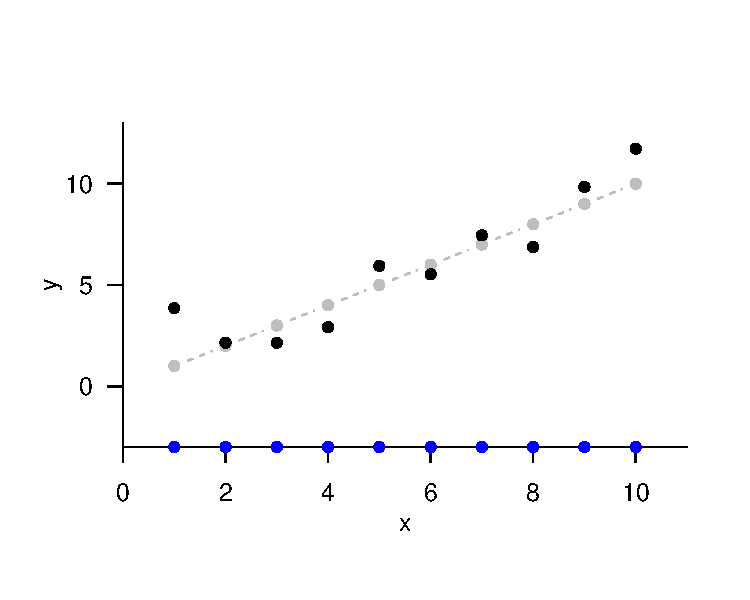
\includegraphics[width=0.8\linewidth]{5_Abbildungen/alm_5_elr} \end{center}
\end{frame}

\begin{frame}{}
\protect\hypertarget{section-11}{}
\large
\setstretch{3}
\vfill

Allgemeine Theorie

Unabhängige und identisch normalverteilte Zufallsvariablen

Einfache lineare Regression

\textbf{Selbstkontrollfragen} \vfill
\end{frame}

\begin{frame}{Selbstkontrollfragen}
\protect\hypertarget{selbstkontrollfragen}{}
\footnotesize
\setstretch{2.5}

\begin{enumerate}
\tightlist
\item
  Erläutern Sie das naturwissenschaftliche Paradigma.
\item
  Erläutern Sie die Standardprobleme der Frequentistischen Inferenz.
\item
  Geben Sie die Definition des Allgemeinen Linearen Modells wieder.
\item
  Erläutern Sie die deterministischen und probabilistischen Aspekte des
  ALMs.
\item
  Wieviele skalare Parameter hat das ALM mit sphärischer
  Kovarianzmatrix?
\item
  Warum sind die Komponenten des ALM Zufallsfehlers unabhängig und
  identisch verteilt?
\item
  Geben Sie das Theorem zur Datenverteilung des Allgemeinen Linearen
  Modells wieder.
\item
  Sind die Komponenten des ALM Datenvektors immer unabhängig und
  identisch verteilt?
\item
  Schreiben Sie das Szenario von \(n\) unabhängig und identisch
  normalverteilten Zufallsvariablen in ALM Form.
\item
  Schreiben Sie das Szenario der einfachen linearen Regression in ALM
  Form.
\end{enumerate}
\end{frame}

\end{document}
